\documentclass[12pt, letter-paper]{article}
\usepackage[utf8]{inputenc}
\usepackage[spanish]{babel}
\usepackage[english]{babel}
\usepackage{graphicx}
\usepackage{float}
\usepackage[left = 2.58 cm, right = 2.58cm, top = 2.58 cm]{geometry}
\usepackage{amsfonts}
\usepackage{amsmath}
\usepackage{amssymb}
\usepackage{multicol}
\usepackage{changepage}
\usepackage{cite}
\usepackage{lipsum}
\usepackage{afterpage}
\usepackage{titlesec}
\usepackage[dvipsnames]{xcolor}
\usepackage[latin1]{inputenc}
\usepackage[usenames]{color}
\usepackage{xcolor}
%\definecolor{mypink3}{cmyk}{0, 0.7808, 0.4429, 0.1412}

\begin{document}
%Portada
\begin{titlepage}
    \centering
    \begin{figure}[t]
        \centering
        {
\includegraphics[scale=1, width=1.7 in]{Imag/logoUD.png}\par}
    \vspace{1cm}
    \end{figure}
    {\scshape\huge Cálculo Multivariado \par}
    \vspace{0.5cm}
    {\scshape\large \textbf{Talleres Grupo 4} \par}
    \vfill
    \vspace{3cm}
    {\normalsize \textbf{Integrantes:} \par}
    \vspace{0.5cm}
    {\normalsize \textit{Luis Daniel Hormiga González \:\:\: Cód. 20172020026} \par}
    {\normalsize\textit{Daysi Carolina Yara Pardo \:\:\: Cód. 20172020077} \par}
    {\normalsize \textit{Juan Camilo Herrera Gómez \:\: Cód. 20191020018} \par}
    {\normalsize \textit{Juan Sebastián Garzon \:\:\: Cód. 20191020068} \par}
    {\normalsize \textit{Juan Nicolas Carmona Vélez \:\: Cód. 20191020096} \par}
    \vspace{3cm}
    {\scshape\normalsize{Universidad Distrital Francisco José De Caldas \\Facultad de Ingeniería \\Bogotá D.C \\ Octubre 2020 \par}}
    \vfill
\end{titlepage}

%Inicio taller
\newpage
\Large{\textcolor{red}{\section{Funciones Vectoriales}}}
\vspace{0.7cm}
\begin{enumerate}
    
    %Primer punto del taller No 4
    \item [$4)$]
    \normalsize{\textbf{Sea}} \par
    \Large{\centering{\textbf{$\vec{r}(t)=\frac{2t}{1+t^{2}}\vec{i}+\frac{1-t^{2}}{t^{2}+1}\vec{j}+\vec{k}$}}\par}
    \vspace{0.5cm}    
    \normalsize{\textbf{Demostrar que el ángulo formado por $\textcolor{red}{\vec{r}(t)\:\:}  y \:\:   \textcolor{red}{\vec{r'}(t)}$ siempre es constante.}}\par
    \vspace{0.5cm}
    \large{\textcolor{red}{Solución}\par}
    \vspace{0.5cm}
    \large{$\vec{r}(t)=\left ( \frac{2t}{1+t^{2}},\frac{1-t^{2}}{t^{2}+1},1 \right )$}\par
    \vspace{0.5cm}
    \large{$\vec{r'}(t)=\left ( \frac{(1+t^{2})2-2t(2t)}{\left({1+t^{2}}\right)^{2}}\:,\frac{(t^{2}+1)(-2t)-(1-t^{2})(2t)}{\left({t^{2}+1}\right)^{2}},0 \right )$}
    \large{$=\left ( \frac{2-2t^{2}}{\left({t^{2}+1}\right)^{2}},\frac{-4t}{\left({t^{2}+1}\right)^{2}},0 \right )$}\par
    \vspace{0.5cm}
    \normalsize{Hallando el ángulo entre $\textcolor{Red}{\vec{r}(t)\:} y \:\: \textcolor{red}{\vec{r'}(t)}$\: usando la ecuación del \textit{ángulo entre dos vectores:}\par}
    \vspace{0.5cm}
    
    %Ecuacion ángulo entre 2 vectores
    \large{\centering {\fboxrule=0.6pt \fcolorbox{Red}{white}{\framebox[5cm] [c]{{$\textcolor{Red}{\theta=cos^{-1}\left( \frac{u\cdot{v}}{\left | u \right |\left | v \right |} \right)}$}}}\par}}
    \vspace{0.5cm}
    \large{$\vec{r}(t)\cdot\vec{r'}(t)=\left(\frac{2t}{t^{2}+1}\right)\left(\frac{2-2t^{2}}{(t^{2}+1)^{2}}\right)+\left(\frac{1-t^{2}}{t^{2}+1}\right)\left(\frac{-4t}{(t^{2}+1)^{2}}\right)$}\par
    \vspace{0.5cm}
    \large{$\vec{r}(t)\cdot\vec{r'}(t)=\frac{4t-4t^{3}}{(t^{2}+1)^{3}}+\frac{4t^{3}-4t}{(t^{2}+1)^{3}}$}\par
    \vspace{0.5cm}
    \large{$\vec{r}(t)\cdot\vec{r'}(t)=\frac{4t-4t^{3}+4t^{3}-4t}{(t^{2}+1)^{3}}\: =\frac{0}{(t^{2}+1)^{3}}\:=0$}\par
    \vspace{0.5cm}
    \large{$\theta=cos^{-1}\left( \frac{0}{\left | r \right |\left | r' \right |} \right)  =cos^{-1}\left( 0 \right)$}\par
    \vspace{0.5cm}
    \large{$\theta=90^{\circ}$}\par
    \vspace{0.5cm}
    \normalsize{\textcolor{Red}{\textbf{Conclusión:}\:}Al obtener un ángulo de $90^{\circ}$, se concluye que el ángulo formado por $\textcolor{Red}{\vec{r}(t)\:} y \:\: \textcolor{red}{\vec{r'}(t)}$ es constante para cualquier \textit{t}}
    \vspace{1cm}
    
    %Segundo punto del taller No 8
    \item [$8)$]
    \normalsize{\textbf{Calcular \textcolor{Red}{$\Vec{r}(t) \cdot \Vec{u}(t)$} siendo $\vec{r}(t)= 2\vec{i}-4\vec{j}+4\vec{k}\:\:$ y $\:\:\vec{u}(t)= \int_{0}^{1}\left ( te^{t}\vec{i}+tcosh2t\vec{j}+te^{-2t}\vec{k} \right )dt$}} \par
    \vspace{0.5cm}
    \large{\textcolor{red}{Solución}\par}
    \vspace{0.5cm}
    \normalsize{\centering{$\vec{r}(t)= 2\vec{i}-4\vec{j}+4\vec{k}\:\:$ y $\:\:\vec{u}(t)= \int_{0}^{1}\left ( \textcolor{Sepia}{te^{t}\vec{i}}+\textcolor{WildStrawberry}{tcosh2t\vec{j}}+\textcolor{NavyBlue}{te^{-2t}\vec{k}}\right )dt$\par}} 
    \vspace{0.5cm}
    \normalsize{Se resuelve \large{$\:\vec{u}(t)$}:}\par
    \vspace{0.5cm}
    $\vec{u}(t)= \int_{0}^{1} te^{t}\:dt+ \int_{0}^{1} tcosh2t\:dt+ \int_{0}^{1} te^{-2t}\:dt$
    \vspace{0.5cm}
    \begin{enumerate}
        % a)
        \item{\textcolor{Sepia}{$\int_{0}^{1} te^{t}\:dt$}} \par
        \normalsize{\centering{\begin{tabular}{r l}
                    $u=t & dv=e^{t} \\
                   \\ du=1 & v=e^{t}$
                    \end{tabular}}\par}
        $\\\int_{0}^{1} te^{t}\:dt=te^{t}-\int{e^{t}}dt$
        \vspace{0.7cm}
        $\\=te^{t}-e^{t}\mid_{0}^{1}\:$\par
        $\\=e^{t}(t-1)\mid_{0}^{1}\:\\$\par
        $=e^{1}(1-1)-[e^{0}(0-1)]=1 \:\textcolor{Red}{\Rightarrow  \vec{u}(t)\vec{i}}$
        \vspace{0.5cm}
        % b)
        \item {\textcolor{WildStrawberry}{$\int_{0}^{1} tcosh2t\vec{j}\:dt$}}\par
        \normalsize{\centering{\begin{tabular}{r l}
                    $u=t & dv=cos(2t) \\
                   \\ du=1 & v=\tfrac{1}{2}senh(2t)$
                    \end{tabular}}\par}
        \vspace{0.7cm}
        $\\\int_{0}^{1} tcosh2t\vec{j}\:dt=\tfrac{t}{2}senh(2t)-\tfrac{1}{2}\int{senh(2t)}dt$
        \vspace{0.5cm}
        $\\=\tfrac{t}{2}senh(2t)-\tfrac{1}{4}cosh(2t)\mid_{0}^{1}\:\\$\par
        $=\tfrac{t}{2}\left(tsenh(2t)-\tfrac{1}{2}cosh(2t)\right)\mid_{0}^{1}\:$\par
        $\\=\frac{e^{4}-3}{8e^{2}}+\frac{1}{4} \:\textcolor{Red}{\Rightarrow \vec{u}(t)\vec{j}}$
        \vspace{0.5cm}
        % c)
        \item {\textcolor{NavyBlue}{$\int_{0}^{1} te^{-2t}\vec{k}\:dt$}}\par
        \normalsize{\centering{\begin{tabular}{r l}
                    $u =t & dv = e^{-2t} \\
                    \\du =1 & v = -\tfrac{1}{2}e^{-2t}$
                    \end{tabular}}\par}
         \vspace{0.7cm}
         $\\\int_{0}^{1} te^{-2t}\vec{k}\:dt=-\tfrac{t}{2}e^{-2t}+\tfrac{1}{2}\int{e^{-2t}}dt$\par
         $\\=-\tfrac{t}{2}e^{-2t}-\tfrac{1}{4}e^{-2t}\mid_{0}^{1}\:\\$ $\\=-\tfrac{t}{2}e^{-2t}(t+\tfrac{1}{2})\mid_{0}^{1}\:$\par
         $\\=-\tfrac{1}{2}e^{-2}(1+\tfrac{1}{2})-[-\tfrac{1}{2}e^{0}(0+\tfrac{1}{2})]$\par
         $\\=-\tfrac{3}{4}e^{-2}+\tfrac{1}{4} = -\tfrac{1}{4}(3e^{-2}-1)\:\textcolor{Red}{\Rightarrow  \vec{u}(t)\vec{k}}$\\\par
        
        \normalsize{Entonces:}\par
        $\\\vec{u}(t)=\left(1,\frac{e^{4}-3}{8e^{2}}+\frac{1}{4},-\tfrac{1}{4}(3e^{-2}-1)\right)$\: y\: $\vec{r}(t)=\left( 2,-4,4\right)$\par
        \vspace{0.5cm}
        \\\normalsize{Resolvemos $\vec{r}(t)\cdot\vec{u}(t)$:}\par
        $\\\vec{r}(t)\cdot\vec{u}(t)= 2(1)+\left(-4\left(\frac{e^{4}-3}{8e^{2}}+\frac{1}{4}\right)\right)+4\left(-\tfrac{1}{4}(3e^{-2}-1)\right)$\\
        $\\= 2-\frac{e^{4}-3}{2e^{2}}-1+\left(-1(3e^{-2}-1)\right)$\\
        $\\= 2-\frac{e^{4}-3}{2e^{2}}-1-3e^{-2}+1$\\
        $\\= 2-\frac{e^{4}-3}{2e^{2}}-3e^{-2}$\\
        $\\= 2-\frac{e^{4}-3}{2e^{2}}-\frac{3}{e^{2}} = 2-\frac{e^{4}-3}{2e^{2}}-\frac{6}{2e^{2}}$\\
        $\\= 2-\frac{e^{4}-3-6}{2e^{2}} = 2-\frac{e^{4}-9}{2e^{2}}$\\
        \\\fboxrule=0.5pt \fcolorbox{Red}{white}{\framebox[5cm] [c]{\textcolor{Red}{$= 2-\frac{(e^{2}-3)(e^{2}+3)}{2e^{2}}$}}}
        
    \end{enumerate}
    \vspace{1.5cm}\par
    
    %Tercer punto del taller No 12
    \item [$12)$]
    \normalsize{\textbf{Supóngase que una partícula sigue la trayectoria \textcolor{Red}{$\vec{r}(t)=\left \langle e^{t},e^{-t},cost \right \rangle$\:}hasta que sale por la tangente en \textit{t=1}, ¿donde estará en \textit{t=3}?}\par}
    \vspace{0.5cm}
    \large{\textcolor{red}{Solución}\par}
    \vspace{0.5cm}
                    \begin{tabular}{r l}
                    $\vec{r}(t)=\left (e^{t},e^{-t},cost \right);$ &  \:\:t_{0} = 1  \\
                    \\$\vec{r'}(t)=\left (e^{t},-e^{-t},-sent \right);$ &   \:\: t_{1} = 3
                    \end{tabular}\par
    \vspace{1cm}
    $\\r_{0}=\vec{r}(1)=\left (e^{1},e^{-1},cos(1) \right)$\\    
    $\\V_{0}=\vec{r'}(1)=\left (e^{1},-e^{-1},-sen(1) \right)$
    \vspace{1cm}
    \\\normalsize{Parametrizamos la recta con la fórmula de la posición:}\par
    \begin{center}
        \large{\fboxrule=0.5pt \fcolorbox{Red}{white}{\framebox[5cm] [c]{\textcolor{Red}{$X_{1}=X_{0}+\Delta t\vec{v}$}}}}   
    \end{center}
    \par
    $\\X=r_{0}+(t_{1}-1)V_{0}$\\
    $\\=\left (e^{1},e^{-1},cos(1)\right)+(t_{1}-1)\left (e^{1},-e^{-1},-sen(1)\right)$\\    
    $\\=\left (e^{1},e^{-1},cos(1)\right)+(3-1)\left (e^{1},-e^{-1},-sen(1)\right)$\\    
    $\\=\left (e^{1},e^{-1},cos(1)\right)+(2)\left (e^{1},-e^{-1},-sen(1)\right)$\\    
    $\\=\left (e^{1},e^{-1},cos(1)\right)+\left (2e^{1},-2e^{-1},-2sen(1)\right)$\\    
    \par
    \normalsize{\fboxrule=0.5pt \fcolorbox{Red}{white}{\framebox[8cm] [c]{\textcolor{Red}{$=\left (3e^{1},-e^{-1},cos(1)-2sen(1)\right)$}}}}
    
    % Cuarto punto del taller No 21
    \newpage
     \item [$21)$]
     \normalsize{\textbf{Determine el punto de la curva}}\par
     \vspace{0.5cm}
     \normalsize{\centering{\textbf{$\vec{r}(t)=\left(5sent\right)\vec{i}+\left(5cost\right)\vec{j}+12t\vec{k}$}}\par}
     \vspace{0.5cm}
     \normalsize{\textbf{Que se encuentra a una distancia de $\textcolor{Red}{26\pi}$  unidades desde el origen a lo largo de la curva, en la direccción en la que crece la longitud de arco. }\par}
     \vspace{0.5cm}
    \large{\textcolor{red}{Solución}}
    \vspace{0.5cm}
    $\\r(t) = (5sen(t))\vec{i} + (5cos(t))\vec{j} + 12t\vec{k}$
    \vspace{0.5cm}
    $\\r'(t) = (5cos(t))\vec{i} - (5sen(t))\vec{j} + 12\vec{k}$
    \vspace{0.5cm}
    $\\26\pi= \int_{0}^{T}\sqrt{25cos^2(t) + 25sen^2(t)+12^2} dt$
    \vspace{0.5cm}
    $\\26\pi= \int_{0}^{T}\sqrt{25+144} dt$
    \vspace{0.5cm}
    $\\26\pi= \int_{0}^{T}\sqrt{169} dt$
    \vspace{0.5cm}
    $\\26\pi= \int_{0}^{T}13 dt$
    \vspace{0.5cm}
    $\\26\pi= 13T$
    \vspace{0.5cm}\par
    \normalsize{Ahora, despejando \textcolor{Red}{T:}}
    \vspace{0.5cm}
    \large{$\\26\pi= 13T$}
    \vspace{0.5cm}
    $\\26\pi - 13T = 0$
    \vspace{0.5cm}
    $\\13(2\pi-T) = 0\rightarrow (2\pi-T) = 0\rightarrow T=2\pi$
    \vspace{0.5cm}\par
    \normalsize{Entonces:}
    \vspace{0.5cm}
    \large{$\\r(2\pi) = ((5sen(2\pi)) , (5cos(2\pi)) , 12(2\pi)) = (0 , 5, 24\pi)$}
    \vspace{1cm}
    
    % Quinto punto del taller No 27
    \item [$27)$]
    \normalsize{\textbf{Grafique las curvas trazadas por las siguientes funciones vectoriales:}\par}
    \begin{enumerate}
      \textbf{\item{$\vec{r}(t)=ti+2tj+costk,\:\:\:\: t\geqslant 0$} 
        \item {$\vec{r}(t)=ti+t^{2}j+tk$}
        \item {\normalsize{La función vectorial que describe la curva intersección entre el plano \textcolor{Red}{$y=2x$}} con el paraboloide \textcolor{Red}{$z=9-x^{2}-y^{2}$}}}
    \end{enumerate}
    \large{\textcolor{red}{Solución}\par}
    \vspace{0.5cm}
    \subsection*{a) r($t$) = $t$i + 2$t$j + $\cos$ $t$k,  $t$ $\geq$ 0 }
    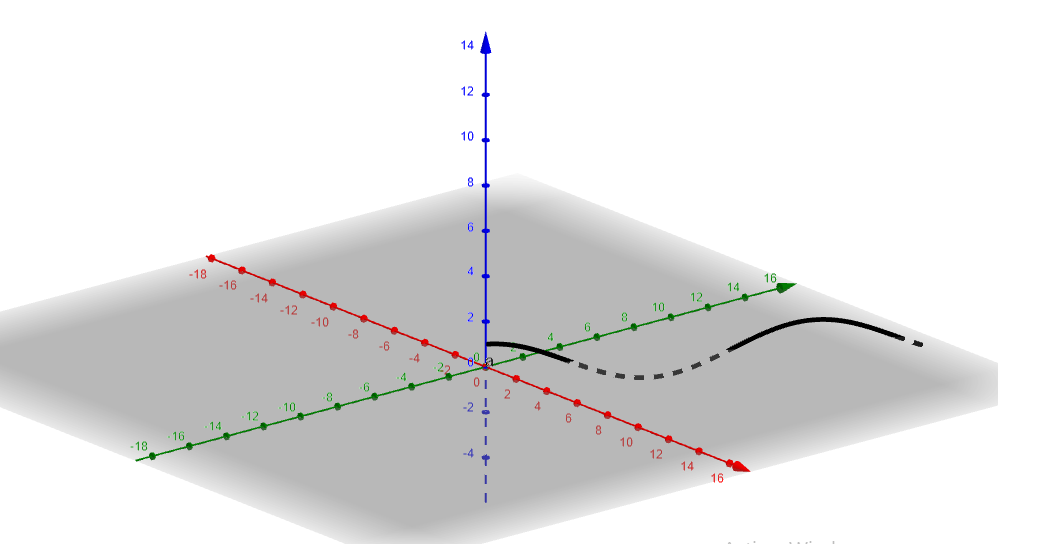
\includegraphics[width=.95\textwidth]{Imag/27-a.png}
    \subsection*{b) r($t$) = $t$i + $t^2$j + $t$k}
    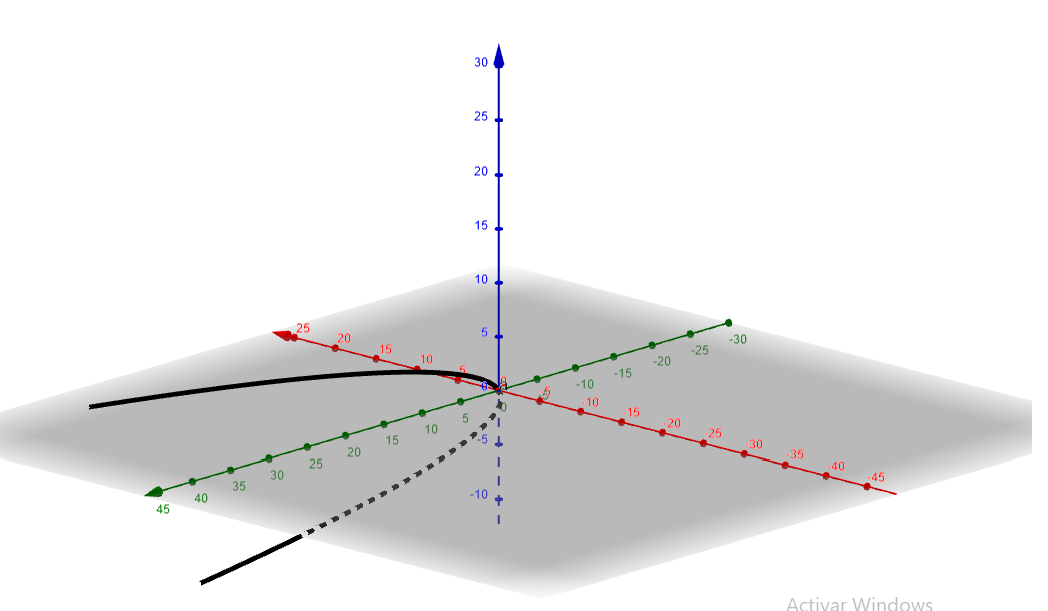
\includegraphics[width=.95\textwidth]{Imag/27-b.png}
    \subsection*{c) la funcion vectorial que describe la curva interseccion entre el plano $y=2x$ con el paraboloide $z=9-x^2-y^2$}
    
    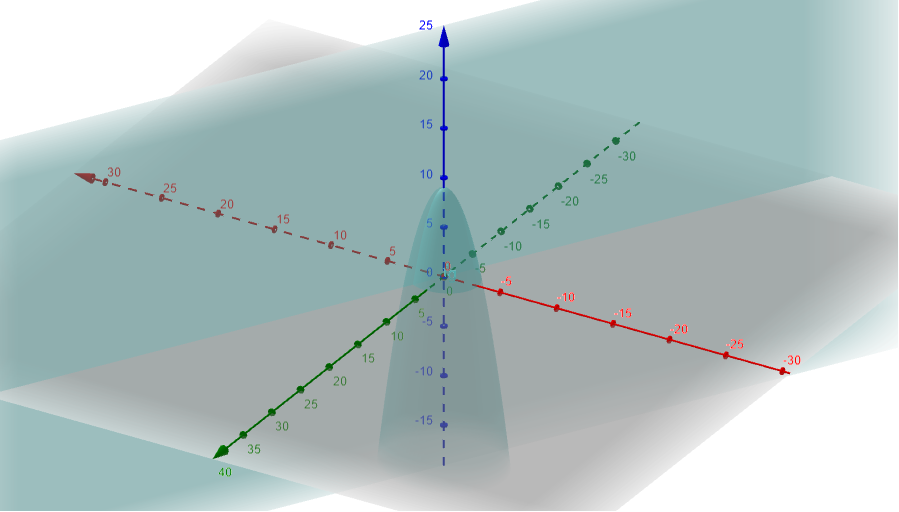
\includegraphics[width=0.95\textwidth]{Imag/27-c1.png} 
    \begin{center}
    $\left\{\begin{array}{c}{y=2x} \\ {z=9-x^2-y^2}\end{array}\right.$
    \end{center} 
    \begin{center}
    $\rightarrow z=9-x^2-(2x)^2$\\$z=9-x^2-4x^2$\\$z=9-5x^2$
    \end{center}
    \begin{center}
    $x(t)=t$\\$y(t)=2t$\\$z(t)=9-t^2$
    \end{center}
    \begin{center}
    r($t$)=$t$i + $2t$j $9-t^2$k
    \end{center}
    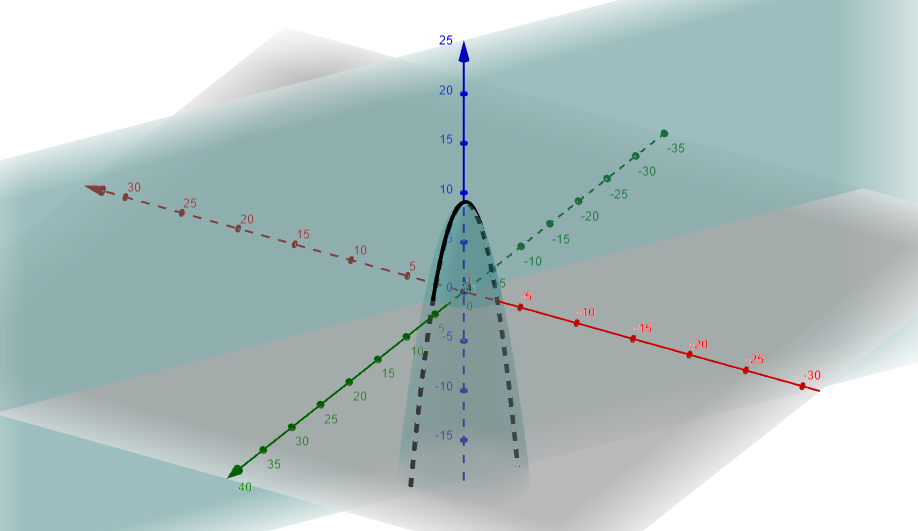
\includegraphics[width=.95\textwidth]{Imag/27-c.png}

    

\end{enumerate}
\end{document}